\documentclass[oneside]{book}
\usepackage{preamble}

\begin{document}
\frontmatter
\thispagestyle{empty}
\AddToShipoutPicture*{}
{\HUGE \textsf{\\ Also sprach \\ Marc Schaul}}

{\huge \textsf{\\Mathe für alle und keinen}}

\vspace{1em}
{\Large \noindent Thomas \textsc{Arocena} \\ Constance \textsc{Sarrazin} \\ Marc \textsc{Schaul} (apocryphe)}
\vfill
\epigraph{\large «~Une exposition très claire, presque éblouissante. Je n'ai jamais lu quoi que ce soit d'aussi brillant depuis mon arrivée en sup 4.~»}{\Large --- Marc Schaul (probablement)}
\epigraph{\large «~Vous savez, ce n'est pas parce que vous ajoutez des «~probablement~» que vous pouvez me faire dire tout et n'importe quoi !~»}{\Large --- Marc Schaul (probablement)}
\newpage
\tableofcontents

\addtocontents{toc}{Le niveau d'une section est indiqué par sa couleur : verte quand sa quasi-entiereté est au programme (officiel ou officieux) des classes préparatoires (MPSI/MP) ; bleue quand son contenu est directement accessible à un spé sans être au programme, autrement dit, quand tous ses préliminaires sont verts ; rouge pour les divagations au delà. 

\medskip

Les items grisés signalent une section en cours de rédaction. L'ensemble est en amélioration constante et comporte selon toute probabilité des erreurs graves. Pour toute réclamation, merci de frapper Thomas (mais pas trop fort histoire qu'il puisse quand même passer les concours)

\medskip

On a veillé à ce que l'ensemble ne soit pas circulaire, mais cela ne veut pas dire que nous avons évité les références en avant, au contraire. Nous nous sommes affranchis de l'ordre linéaire sans scrupule lorsque cela était nécessaire. En particulier, les sections rouges piochent librement dans le contenu des sections vertes sans forcément renvoyer aux pages correspondantes.

\medskip

Cette version est celle du \today. Pour accéder à l'historique, faites un tour sur le repo GitHub.\hfill\par}
\mainmatter
\partie{Fourre-tout}{}
\chapter{Théorie des ensembles}
\vspace{-1cm}
\greensection{Une théorie sur des bases frêles}{Une introduction à la terminalogie ensembliste sur le mode dit naïf : unions, intersections, produit cartésien. Algèbre de Boole des parties d'un ensemble. Relations binaires, relations d'ordre, d'équivalence, partition. Applications, injections, surjections, bijections. Argument diagonal de Cantor. Théorème de Schröder-Bernstein.}
\subsection*{Premières opérations ensemblistes}
On considère ici qu'un ensemble est un concept intuitif, qui correspond à une collection d'objets mathématiques. Ces objets sont définis par une propriété ou par une liste exhaustive, de la façon suivante~: 
\begin{itemize}
    \item $\R_+ = \{x\in \R |x\geq 0\}$
    \item $P = \{1,4,9,16\} = \{n \in \N | n \text{ est un carré parfait et } n<20\}$
\end{itemize}
Cette première expression se lit par exemple «~$\R_+$ est l'ensemble des $x$ dans $\R$ tels que $x\geq 0$~».

On verra dans le chapitre suivant que pour éviter d'aboutir à certaines contradictions techniques, il est nécessaire de restreindre quelque peu ce qu'on s'autorise à considérer comme un ensemble. Mais pour le moment, on suppose acquise cette fondation et on introduit un peu de vocabulaire, en commençant par les opérations ensemblistes de base.

\begin{defini}[Union et intersection]
    Soient $A$ et $B$ deux ensembles. 
    
    On note $A\cup B$ l'union de $A$ et $B$, c'est à dire l'ensemble \[\{x|x\in A \text{ ou } x\in B\}\] 
    On note $A\cap B$ l'intersection de $A$ et $B$, c'est à dire l'ensemble \[\{x|x\in A \text{ ou } x\in B\}\]
\end{defini}

Cette situation est bien résumée par un diagramme de Venn :

\medskip
\begin{tikzpicture}
\draw[color=gray] (0,0) rectangle (\textwidth, 2);
\draw[color=cadmiumred] (\textwidth/5, 1) circle (0.8);
\draw[color=cobalt] (\textwidth/10, 1) circle (0.8);
\draw (\textwidth/2, 1) node{Grave la flemme mais l'idée est là};
\draw[color=cadmiumred] (9\textwidth/10, 1) circle (0.8);
\draw[color=cobalt] (4\textwidth/5, 1) circle (0.8);
\end{tikzpicture}

Ces opérations sont la transcription directe du «~et~» et du «~ou~» logique\footnote[1]{Notons que le ou logique, contrairement à certains usages en français, est un ou inclusif : autrement dit, $P$ ou $Q$ signifie que soit $P$ est vrai, soit $Q$ est vrai, soit $P$ et $Q$ sont tous deux vrais. On verra dans quelques pages l'opération ensembliste traduisant le ou exclusif ($P$ ou $Q$ mais pas les deux.)}. On peut donc écrire nos premières propriétés : 

\begin{prop}
    Pour tous ensembles $A$, $B$ et $C$ :
    \begin{multicols}{2}
    \begin{itemize}
        \item $A\cup A=A$
        \item $A\cup B=B\cup A$
        \item $(A\cup B)\cup C = A\cup(B\cup C)$ 
        \item $A\cap(B\cup C)=(A\cap B) \cup (A\cap C)$
        \item $A\cap A=A$
        \item $A\cap B=B\cap A$
        \item $(A\cap B)\cap C = A\cap(B\cap C)$
        \item $A\cup(B\cap C)=(A\cup B) \cap (A\cup C)$
    \end{itemize}
\end{multicols}
    Ces propriétés s'appellent respectivement l'idempotence, la commutativité, l'associativité et la distributivité.
\end{prop}
\begin{demo}
    Ces propriétés proviennent directement des propriétés des opérateurs logiques et et ou. Par exemple, étant donné une proposition $P$, $P$ ou $P$ équivaut à $P$.
\end{demo}

On peut encore faire quelques diagrammes de Venn pour illustrer la situation.

\vfill
\begin{tikzpicture}
\draw[color=gray] (0,0) rectangle (\textwidth, 3.5);
\draw (\textwidth/2, 1.75) node{Toujours pas};
\end{tikzpicture}
\vfill

On peut encore transcrire l'implication logique par la notion de partie.

\begin{defini}[Parties]
    Soit $A$ et $B$ deux ensembles. On dit que $A$ est inclus, contenu dans $B$, ou encore que c'est une partie ou un sous-ensemble de $B$, quand $x\in A \implies x\in B$, c'est à dire $\forall x\in A, x\in B$. On le note $A\subset B$. On notera $\Ps(B)$ l'ensemble de toutes les parties de $B$.
\end{defini}

Par exemple, comme $x\in A \text{ et } x\in B \implies x\in A$, il est facile de se convaincre que $A\cap B$ est une partie de $A$. 
\newpage
De même, comme $x\in A \implies x\in A$, on a toujours $A\subset A$.\footnote[2]{Les anglo-saxons écrivent souvent $\subseteq$ pour l'inclusion telle que nous venons de la définir et réservent $\subset$ à l'inclusion stricte : pour eux, $A\subset B\iff A \subseteq B \text{ and } A\neq B$. On écrira $A \subsetneq$ dans ce cas.}

Un ensemble remarquable est l'ensemble vide, ne comportant aucun élément, qu'on note $\varnothing$ : $x\in\varnothing$ étant toujours faux, l'implication $x\in\varnothing \implies x\in A$ est, elle, toujours vraie, et pour tout ensemble $A$, $\varnothing \subset A$.  

De plus, dans le cas particulier où $A$ est un ensemble avec un nombre fini d'éléments, on peut lister toutes ses parties. Par exemple, l'ensemble $\{1,2\}$ a pour parties~:
\[\varnothing \qquad \{1\} \qquad \{2\} \qquad \{1,2\}\]  
$\Ps(\{1,2\})$ comporte donc 4 éléments.

\begin{prop}
    Soit $E$ un ensemble à $n$ éléments. Alors $\Ps(E)$ comporte $2^n$ éléments.
\end{prop}
\begin{demo}
    Dénombrons toutes les parties de $E$. On peut faire la liste de tous les éléments de $E$, de telle sorte qu'il a un sens de parler du premier élément, du deuxième, etc. On a deux choix pour le premier élément : soit on l'inclut, soit on ne l'inclut pas. De même, on a ensuite deux choix pour le deuxième élément, ce qui nous amène à un total de quatre choix, et ainsi de suite : on aura huit choix au troisième élément et de proche en proche $2^n$ à l'énième.
\end{demo}

Enfin, la négation logique correspond à la notion de complémentaire, et à la notion liée d'ensemble privé d'un autre.

\begin{defini}[Complémentaire et « privé de »]
    Soit $A$ une partie de $B$. On note ${A}_C$ l'ensemble $\{x\in B|x\not\in A\}$. C'est le complémentaire de $A$ dans $B$.

\medskip
    Soient maintenant $A$ et $B$ quelconques. On note $B\backslash A$ et on lit « $B$ privé de $A$ » le complémentaire de $A\cap B$ (qu'on sait être une partie de $B$) dans $B$.

\medskip
    Quand $A$ est une partie de $B$, comme $A\cap B = A$, ces deux notions sont confondues.
\end{defini}

Remarquons que la notation $A_C$ peut être ambiguë si il y a un doute sur l'ensemble de référence : en clair, dans une situation où on manipule trois ensembles $A$, $B$ et $C$ avec $A\subset B \subset C$, $A_C$ peut être le complémentaire de $A$ dans $B$ ou dans $C$. Dans une telle situation, on préférera les notations $B\backslash A$ et $C\backslash A$ qui dissiperont ce doute.

\medskip
Comme précédemment pour les unions et les intersections, on dispose de propriétés permettant de simplifier certaines expressions.

\begin{prop}
    Soient $A$ et $B$ deux parties d'un même ensemble.
\begin{itemize}
    \item $(A_C)_C=A$
    \item $(A\cup B)_C= A_C \cap B_C$
    \item $(A\cap B)_C= A_C \cup B_C$
\end{itemize}    
\end{prop}

Ces deux dernières propriétés s'appellent les lois de De Morgan, et s'illustrent bien par des diagrames de Venn.

\medskip
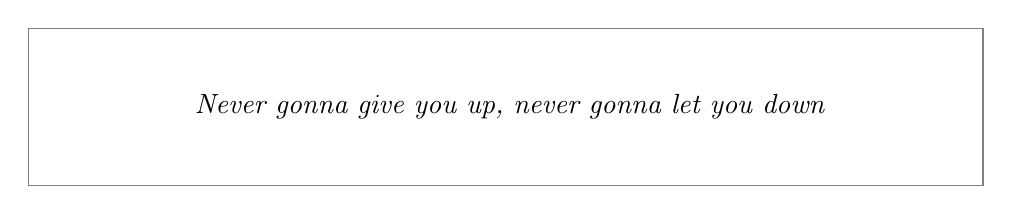
\begin{tikzpicture}
\draw[color=gray] (0,0) rectangle (\textwidth, 2);
\draw (\textwidth/2, 1) node{\eighthnote \textit{ Never gonna give you up, never gonna let you down} \twonotes};
\end{tikzpicture}


\medskip
On peut maintenant définir une opération qui rend compte du « ou exclusif » :
\begin{wrapfigure}[2]{r}{0.33\textwidth}
    \vspace{-0.5em}
    
\begin{tikzpicture}
        \draw[color=gray] (0,0) rectangle (\textwidth/3, 2.1);
        \draw (\textwidth/6, 1.05) node{Hahahahaha};
    \end{tikzpicture}
\end{wrapfigure}

\vspace{-1em}
\begin{defini}
    Soit $A$ et $B$ deux ensembles. On note $A\Delta B$ la différence symétrique de $A$ et $B$ c'est à dire l'ensemble $A\cup B \backslash A\cap B$.
\end{defini}

Enfin, une dernière opération est importante pour la suite : le produit cartésien. 

\begin{defini}
Soient deux ensembles $A$ et $B$. Le produit cartésien $A\times B$ («~A croix B~») est l'ensemble des couples $(a,b)$ où $a$ appartient à $A$ et $b$ appartient à $B$.
\end{defini}

On suppose ici que la notion de couple est intuitive\footnote{Cela dit, on peut aussi définir un couple d'une façon purement ensembliste, par exemple en posant $(a,b)=\{a, \{a, b\}\}$. Une telle définition permet d'identifier le premier élément, mais elle peut sembler artificielle à ce stade.} : il s'agit d'une paire ordonnée, contrairement à un ensemble à deux éléments qui ne l'est pas. Autrement dit $(a,b)=(a',b')\implies a=a' \text{ et } b=b'$, tandis que $\{a,b\}=\{a',b'\}\implies (a=a' \text{ et } b=b') \text{ ou } (a=b' \text{ et } b=a')$. 

En l'état, $(A\times B)\times C$ et $A\times (B\times C)$ ne sont pas égaux, mais une fois qu'on disposera d'une définition du produit cartésien d'une famille d'ensembles, on pourra identifier ces deux ensembles à $A\times B \times C$. 

Pour le moment ceci n'est pas très important, et on peut provisoirement se restreindre à des situations mettant en jeu le produit simple de deux éléments. En particulier, ceci suffit pour définir les relations binaires.

\subsection*{Relations binaires et d'ordre}
D'un point de vue logique, une relation binaire entre deux objets est comparable à une fonction -- au sens informatique du terme -- prenant deux arguments et renvoyant une valeur logique, vrai ou faux. Ceci correspond en général à l'introduction d'un nouveau symbole. Par exemple, l'égalité, l'appartenance d'ensembles, l'inclusion d'ensembles sont des relations binaires.

D'un point de vue ensembliste, ceci correspond à la donnée d'un sous-ensemble :
\begin{defini}
    Une relation binaire $\mathcal{R}$ entre éléments de $X$ et de $Y$ peut être vue comme un sous-ensemble $\mathcal{R}$  de produit cartésien $X\times Y$. On notera $x\mathcal{R} y$ pour $(x,y)\in \mathcal{R}$.
\end{defini}

On parlera de relation binaire sur $X$ pour une relation entre éléments de $X$. 

Un type particulier de relations binaires sont les relations d'ordre, habituellement notées $\leq$.

\begin{defini}
    Une relation binaire sur un ensemble $X$ est une relation d'ordre $\leq$ sur $X$ quand :
    \begin{itemize}
        \item réflexive : $\forall x\in X, x\leq x$
        \item antisymétrique : $\forall x,y \in X, x \leq y \text{ et } y \leq x \implies x=y$
        \item transitive : $\forall x,y,z \in X, x\leq y \text{ et } y \leq z \implies x\leq z$
    \end{itemize}  
\end{defini}

On peut d'ores et déjà donner un exemple.

\begin{prop}
    Soit $E$ un ensemble. L'inclusion $\subset$ est une relation d'ordre sur $\Ps(E)$.
\end{prop}
\begin{demo}
\begin{itemize}
    \item Il s'agit bien d'une relation binaire, qui correspond à l'ensemble $\{(A,B)\in \Ps(E)^2 | \forall x\in E, x\in A \implies x\in B\}$.
    \item Pour tout ensemble $A$, $A\subset A$.
    \item Si $X\subset Y$ et $Y\subset X$, par double implication, $x \in X \iff x\in Y$. Autrement dit, $X$ et $Y$ ont exactement les mêmes éléments, soit $X=Y$.
    \item Si $x\in X \implies x\in Y$ et $x\in Y \implies x\in Z$, $x\in X \implies x\in Z$. Autrement dit, si $X\subset Y$ et $Y\subset Z$, alors $X\subset Z$.
\end{itemize}
D'où $\subset$ relation d'ordre.
\end{demo}

Remarquons que selon cette définition, la relation $<$ (par exemple sur les entiers) n'est pas une relation d'ordre. Cepandant, on peut définir les relations d'ordre stricte :

\begin{defini}
    Une relation binaire sur un ensemble $X$ est une relation d'ordre strict $<$ sur $X$ quand :
    \begin{itemize}
        \item Elle est irréfléxive : $\forall x, \text{ non } x < x$
        \item Elle est transitive.
    \end{itemize}
\end{defini}

À partir d'une relation d'ordre $\leq$, on définit l'ordre strict correspondant $x<y \iff x\leq y \text{ et } x\neq y$. Réciproquement, à partir d'un ordre strict $<$, on peut poser $x\leq y \iff x<y \text{ ou } x=y$.

[majorant, minorant, yada yada]

\subsection*{Applications, bijections et familles}
On va en fait définir une application comme une certaine relation binaire.

\begin{defini}
    
\end{defini}

\subsection*{Relations d'équivalences et partitions}
Un autre type de relations binaires remarquables sont les relations d'équivalence.

\begin{defini}
    Une relation d'équivalence sur un ensemble $X$ est une relation binaire $\sim$ sur X :
    \begin{itemize}
        \item réflexive,
        \item symétrique : $\forall x \forall y, x\sim y \implies y \sim x$,
        \item transitive.
    \end{itemize}
\end{defini}

Un premier exemple de relation d'équivalence est bien sûr l'égalité. Un autre exemple est donné par les congruences en arithmétique : en particulier si on pose $p \sim q \iff p$ et $q$ ont la même parité, il s'agit d'une relation d'équivalence.

Toute l'utilité de la notion réside en la possibilité de classer tous les éléments en «~paquets~», qui sont les classes d'équivalences :

\begin{defini}
    Soit $x\in X$. On note $\bar{x}$ ou $[x]$ la classe d'équivalence de $x$, qui est l'ensemble $\{y\in X | x\sim y\}$
\end{defini}

Formellement, on dit que les classes d'équivalences forment une partition de $X$ :
\begin{wrapfigure}[2]{r}{0.25\textwidth}
    \vspace{-0.5em}
    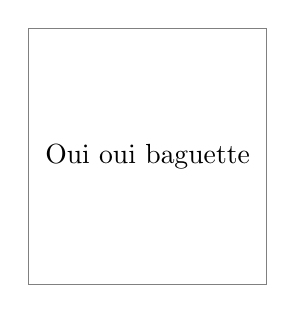
\begin{tikzpicture}
        \draw[color=gray] (0,0) rectangle (\textwidth/4, 3.25);
        \draw (\textwidth/8, 1.625) node{Oui oui baguette};
    \end{tikzpicture}
\end{wrapfigure}

\vspace{-1em}
\begin{defini}
    Soit $X$ un ensemble. On dit que la famille d'ensembles $(X_i)$ forme une partition de $X$ quand :
    \begin{itemize}
        \item $\forall i \in I, X_i \neq \varnothing$
        \item $\bigcup X_i = X$
        \item $\forall i \neq j, X_i \cap X_j = \varnothing$
    \end{itemize}
\end{defini}

\bluesection{Axiomatisation de Zermelo-Frankel (ZFC)}{Paradoxes de Berry, de Russel : axiomes de compréhension, de compréhension restreinte. Classes, correspondances fonctionnelles. Axiome de séparation. Axiomes de l'union, de la paire, de l'ensemble des parties. Bons ordres, ordinaux, cardinaux, leur arithmétique. Axiome du choix, lemme de Zorn, théorème de Zermelo et cardinal de tout ensemble.}

\bluesection{Objets mathématiques usuels et ensembles purs}{Retour sur l'axiome de fondation. Rang, hiérarchie cumulative de Von Neumann, ensemble pur. Construction de copies de $\N$, $\Z$, $\Q$ dans ZFC. Une première construction de $\R$. Application des ordinaux : les suites de Goodstein.}

\partie{Algèbre}{}
\refstepcounter{chapter}
\greensection{Groupes, premières définitions et exemples}{Loi de composition, monoïde, groupe. Morphismes. Sous-groupe, théorème de Lagrange. Ordre d'un élément. Groupe produit, sous-groupe normal et groupe quotient. Exemples : $\Z$, $(\Z/n\Z, +)$, $\mathfrak{S}_n$. Groupe symétrique, signature et théorème de Cayley.}

\greensection{Anneaux et corps, premières définitions et exemples}{Idéal, anneau quotient. Arithmétique dans un anneau intègre : divisibilité, anneaux euclidiens. $\mathbb{Z}$ et $\mathbb{R}[X]$ sont principaux. Relation de Bézout. Éléments irréductibles, premiers, factorisation. Anneau de polynômes. Corps, caractéristique. Corps de fractions. Clôture algébrique et théorème fondamental de l'algèbre. Indicatrice d'Euler et $\mathbb{F}_p$.}

\partie{Topologie}{}
\partie{Analyse}{}
\partie{Théorie des nombres}{}
\partie{Histoire et philosophie}{}
\end{document}